\section*{Problem Statement}
The objective of this problem is to construct and analyze interpolating polynomials using the Lagrange interpolation method. Given a set of data points $(x_i, f(x_i))$, we approximate the function $f(x)$ by polynomials of varying order and compare their behavior. The interpolating polynomials are also used to estimate $f(7)$.

\begin{quote}
  \textbf{NOTE}: The code can be accessed using this link: \href{https://raw.githubusercontent.com/HavokSahil/computational-techniques-assignments/refs/heads/main/assignment3/a1.m}{MATLAB}, \href{https://raw.githubusercontent.com/HavokSahil/computational-techniques-assignments/refs/heads/main/assignment3/a1.jl}{Julia}.
\end{quote}


\section*{Methodology}
The Lagrange interpolation method constructs a polynomial $P_k(x)$ of degree $k$ that passes through $k+1$ data points. It is expressed as:
\[
  P_k(x) = \sum_{i=0}^{k} f(x_i) \, L_i(x),
\]
where the $i^{th}$ Lagrange basis polynomial is given by:
\[
  L_i(x) = \prod_{\substack{j=0 \\ j \neq i}}^{k} \frac{x - x_j}{x_i - x_j}.
\]

This ensures $L_i(x_j) = \delta_{ij}$, so that $P_k(x_j) = f(x_j)$.

\subsection*{Pseudo-code}
\begin{enumerate}
  \item Store the given data points $(X, Y)$.
  \item Define a function to compute the Lagrange basis $L_i(x)$ for a given order $k$.
  \item Define the interpolating polynomial function $P_k(x)$ using the basis functions and data points.
  \item For each order $k = 1, 2, 3$:
    \begin{itemize}
      \item Plot the interpolating polynomial along with the data points.
      \item Evaluate $P_k(7)$ and print the result.
    \end{itemize}
\end{enumerate}

\section*{Results}
The given dataset is:
\[
\begin{aligned}
(x, f(x)) = \{ &(0.5,\, 1.625), (1.5,\, 5.875), (3.0,\, 31.0), \\
               &(5.0,\, 131.0), (6.5,\, 282.125), (8.0,\, 521.0) \}.
\end{aligned}
\]

Interpolating polynomials of order $1, 2,$ and $3$ were constructed. The figure below shows the data points and the interpolated curves.

\begin{figure}[h!]
  \centering
  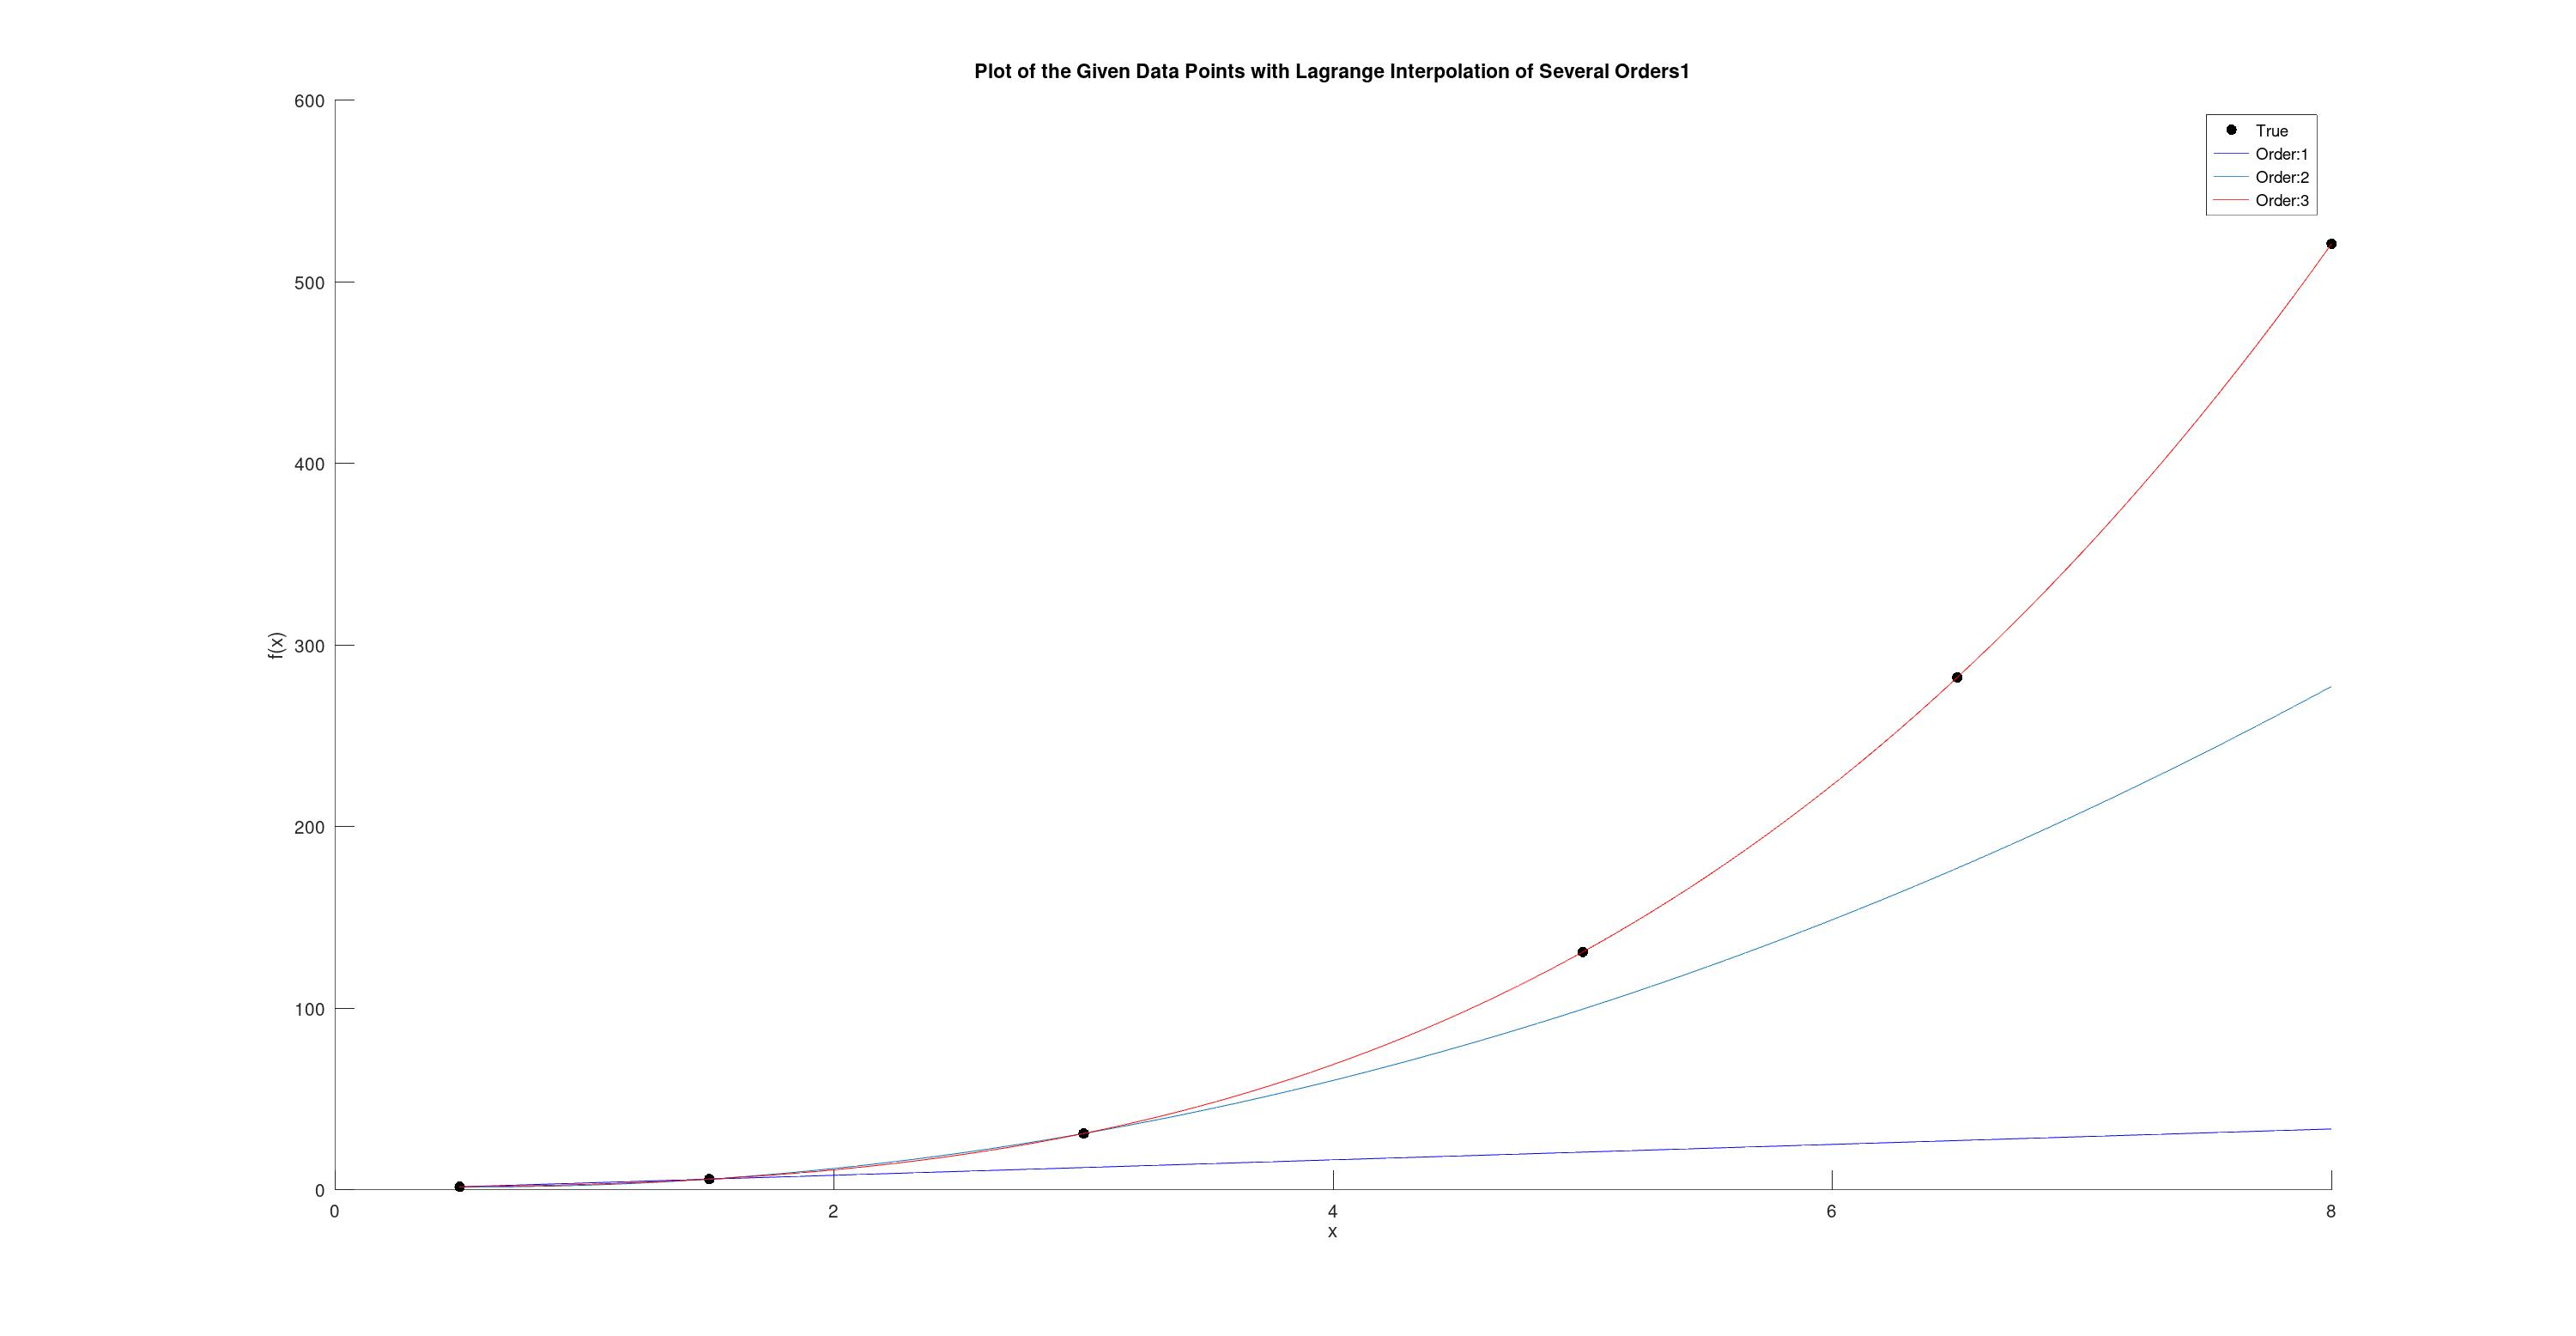
\includegraphics[width=1.0\textwidth]{a1.jpg}
  \caption{Interpolating Functions for Different Orders of Interpolation}
  \label{fig:a1}
\end{figure}

The computed estimates of $f(7)$ are:
\[
\begin{aligned}
  P_1(7) &= \, 29.250000 \\
  P_2(7) &= \, 208.000000 \\
  P_3(7) &= \, 351.000000
\end{aligned}
\]

\section*{Conclusion}
The Lagrange interpolation method was successfully applied to approximate the function given discrete data points. Lower-order polynomials (e.g., $k=1$) provide rough estimates and do not capture the curvature well, while higher-order polynomials fit the data more accurately. The evaluation of $f(7)$ demonstrates how increasing the order improves approximation quality. However, very high-order polynomials may suffer from oscillations (Runge’s phenomenon), so the choice of order must balance accuracy and stability.
